
\documentclass[template=tabling,81pt,headonall]{azmoon}
\usepackage{xepersian}
\usepackage{amsfonts}
\usepackage{graphicx}
\graphicspath{ {./images/} }
\settextfont{Yas}
\setdigitfont{A Iranian Sans}

\printanswers
    \teacher{محمد صالح علی اکبری}
    \teachertitle{دبیر}
    \city{گناباد}
    \schooltitle{متوسطه دوره دوم}
    \school{شهید رجایی}
    \grade{یازدهم}
    \branch{-}
    \topic{ریاضی}
    \examdate{24 مرداد 1402}
    \answertime{90 دقیقه}
    \begin{document}
	\begin{questions}
		\nointerlineskip%
		\vskip-\baselineskip
		\question[2]{%
جدول زیر را کامل کنید. \\ 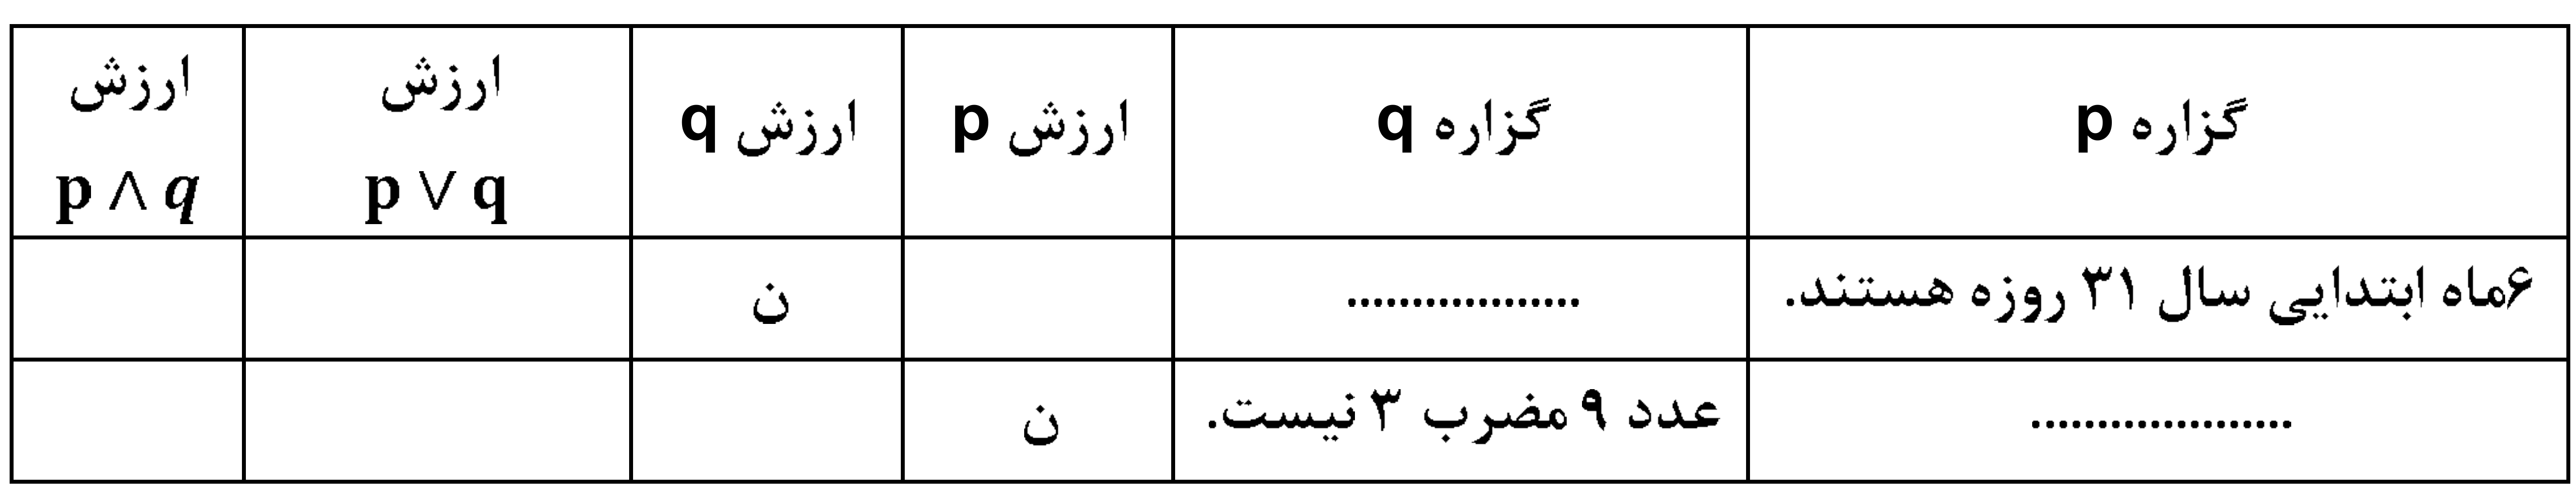
\includegraphics[scale = 1]{جدول_گزاره‌ها}}\question[1]{%
5 افراز مختلف از مجموعه $A = \{1,2,3,4\}$ را بنویسید.
\\
\\}\question[1]{%
اگر $A = \mathbb{N}$ و $B = [1,4]$ باشد مطلوب است نمودار حاصل از ضرب‌های $A \times B$ و $B \times A$.
\\
\\
\\
\\}\question[1.5]{%
اگر $p(A) = \dfrac {2}{5}$ ، $P(B') = \dfrac {3}{7}$ و $P(A \cap B) = \dfrac{1}{5}$ مطلوب است: 
    \begin{LTR}
        \begin{parts}\part{$P(A-B)$}
\part{$P(A \cup B)$}
\end{parts}
\end{LTR}
        
    }\question[1.5]{%
در پرتاب یک سکه ناسالم، احتمال آمدن رو، نصف احتمال آمدن پشت است. در پرتاب این سکه احتمال ظاهر شدن «رو» و احتمال ظاهر شدن «پشت» را بدست آورید.
\\
\\}\question[1.5]{%
در یک شرکت بسته بندی کالا، درصد محصولات تولیدی با سه دستگاه A و B و C به ترتیب 30، 45 و 25 است. اگر 1 درصد محصولات A و 2 درصد محصولات B و 4 درصد محصولات C معیوب باشند و یک کالا به تصادف از بین محصولات شرکت انتخاب کنیم، احتمال اینکه کالا سالم باشد چقدر است؟
\\
\\
\\
\\}\question[2]{%
احتمال آنکه امیر در کنکور قبول شود $0.7$ و احتمال آنکه علی در کنکور قبول شود $0.6$ می‌باشد. مطلوب است احتمال آنکه:
    \begin{parts}\part{هیچکدام از آن‌ها در کنکور قبول نشوند؟}
\part{فقط یکی از آن‌ها در کنکور قبول شوند؟}
\end{parts}
‌
\\‌
\\‌
\\
    }\question[1.5]{%
در یک امتحان تستی 4 گزیه‌ای 10 سؤال مطرح شده است. اگر دانش‌آموزی به همه سؤالات پاسخ دهد. احتمال حالت‌های زیر را بدست بیاورید.: (نیازی به محاسبه جواب آخر نیست)
    \begin{parts}\part{اجتمال پاسخ صحیح به همه سؤالات.}
\part{احتمال پاسخ صحیح به نیمی از سؤالات.}
\end{parts}
‌
\\‌
\\‌
\\‌
\\
    }\question[1]{%
جدول زیر درصد فراوانی نسبی گروه خونی افراد یک جامعه است. در نمودار دایره‌ای، زاویه سطح مربوط به گروه خونی O چند است؟  \\ 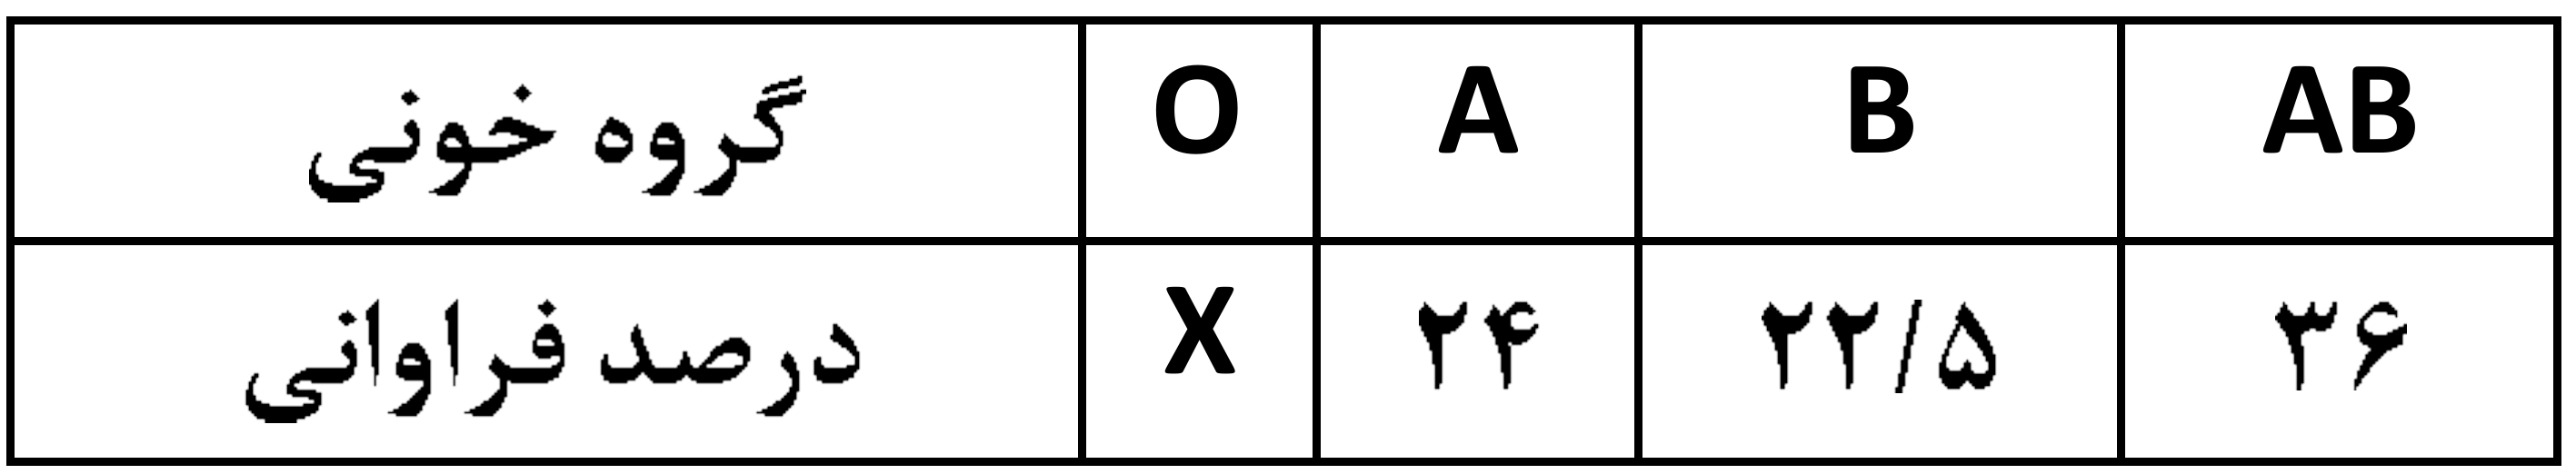
\includegraphics[scale = 1]{جدول_فراوانی_نمودار_دایره‌ای}
\\
\\}\question[1]{%
طبق نمرات زیر معدل دانش‌آموزان کلاسی در درس آمار $16.95$ است. نمره دانش‌آموزی که با x‌نشان داده شده است را محاسبه کنید. \\ X , $17.5$, 19, 17, 16, 20, 16, 15, 18,18
\\
\\}\question[1]{%
در جدول فراوانی مقابل به تمام داده‌ها $1.5$ واحد اضافه می‌شود، میانگین داده‌های جدید ۱۰ می‌شود. فراوانی دسته سوم چقدر است؟ \\ 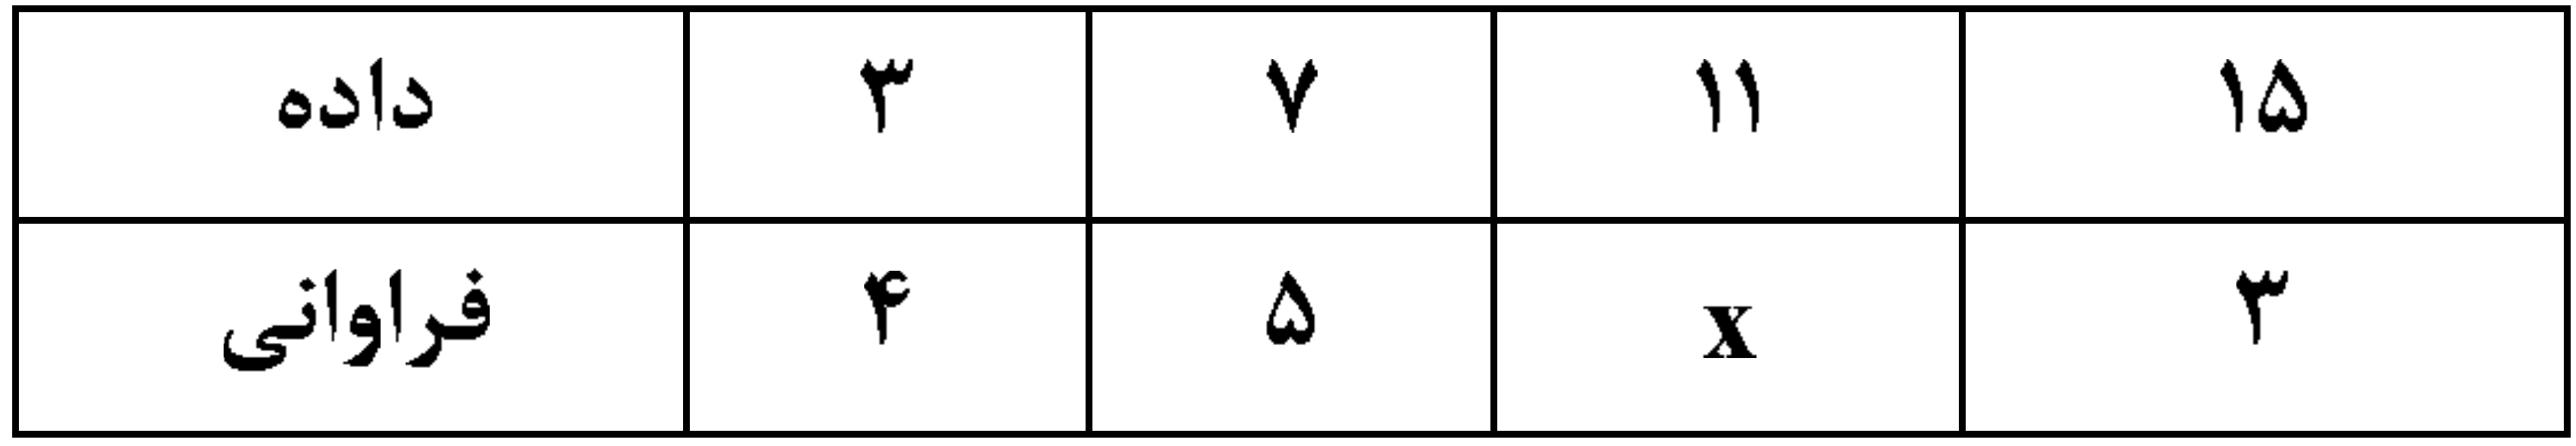
\includegraphics[scale = 1]{جدول_فراوانی_s11}
\\}\question[1.5]{%
برای اعداد زیر، واریانس، انحراف معیار، ضریب تغییرات را بدست بیاورید. \\ 63 ، 50 ، 64 ، 23 ، 45 ، 17 ، 74 ، 53 ، 26 ، 59 ، 32
\\
\\
\\
\\}\question[2]{%
نمودار حعبه‌ای داده‌های زیر را رسم کنید. \\ 2 ، 1 ، 5 ، 5 ، 2 ، 2، 2 ، 2 ، 3 ، 1 ، 1 ، 1 ، 2, 4, 7, 1, 4, 6, 8, 3, 4, 7
\\
\\
\\
\\}\question[0.5]{%
فرق بین داده و متغیر چیست؟
\\
\\}\question[1]{%
اصطلاحات زیر را تعریف کنید.
    \begin{parts}\part{نمونه گیری سیستماتیک}
\part{نمونه گیری تصادفی ساده.}
\end{parts}

    }\end{questions}
    \end{document}
    